% This file was created by tikzplotlib v0.8.5.
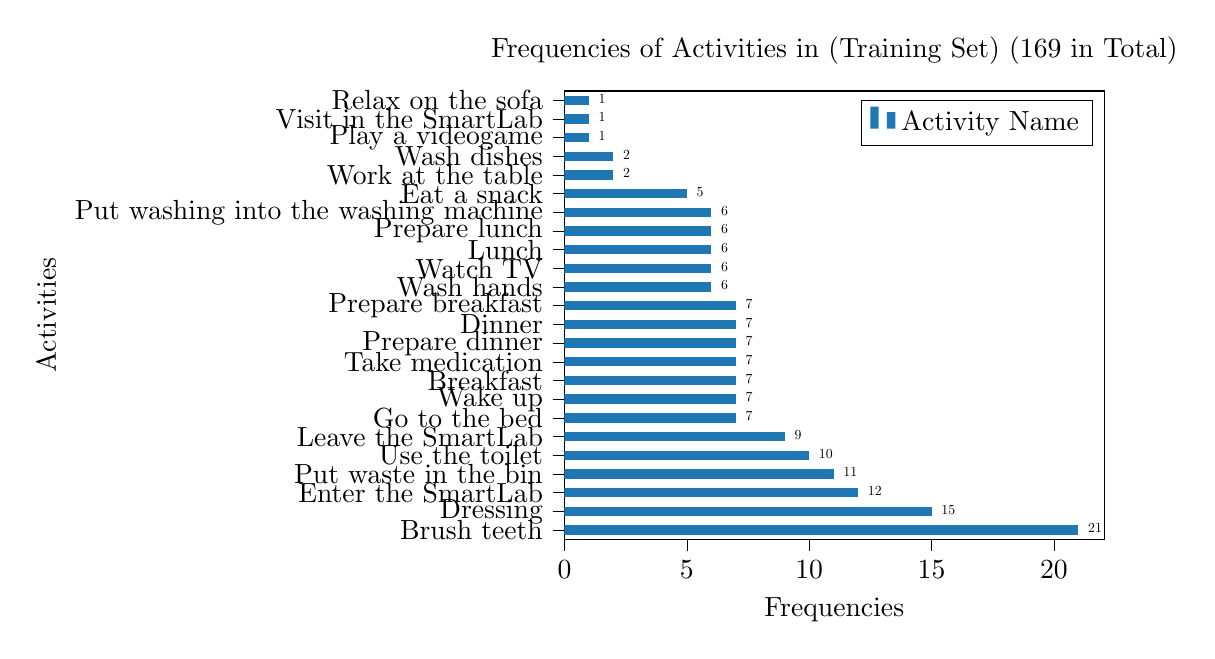
\begin{tikzpicture}

\definecolor{color0}{rgb}{0.12156862745098,0.466666666666667,0.705882352941177}

\begin{axis}[
tick align=outside,
tick pos=left,
title={Frequencies of Activities in (Training Set) (169 in Total)},
x grid style={white!69.01960784313725!black},
xlabel={Frequencies},
xmin=0, xmax=22.05,
xtick style={color=black},
y grid style={white!69.01960784313725!black},
ylabel={Activities},
ymin=-0.5, ymax=23.5,
ytick style={color=black},
ytick={0,1,2,3,4,5,6,7,8,9,10,11,12,13,14,15,16,17,18,19,20,21,22,23},
yticklabels={Brush teeth,Dressing,Enter the SmartLab ,Put waste in the bin ,Use the toilet,Leave the SmartLab,Go to the bed,Wake up,Breakfast,Take medication ,Prepare dinner ,Dinner,Prepare breakfast,Wash hands,Watch TV,Lunch,Prepare lunch,Put washing into the washing machine,Eat a snack,Work at the table ,Wash dishes,Play a videogame ,Visit in the SmartLab ,Relax on the sofa }
]
\draw[fill=color0,draw opacity=0] (axis cs:0,-0.25) rectangle (axis cs:21,0.25);
\addlegendimage{ybar,ybar legend,fill=color0,draw opacity=0};
\addlegendentry{Activity Name}

\draw[fill=color0,draw opacity=0] (axis cs:0,0.75) rectangle (axis cs:15,1.25);
\draw[fill=color0,draw opacity=0] (axis cs:0,1.75) rectangle (axis cs:12,2.25);
\draw[fill=color0,draw opacity=0] (axis cs:0,2.75) rectangle (axis cs:11,3.25);
\draw[fill=color0,draw opacity=0] (axis cs:0,3.75) rectangle (axis cs:10,4.25);
\draw[fill=color0,draw opacity=0] (axis cs:0,4.75) rectangle (axis cs:9,5.25);
\draw[fill=color0,draw opacity=0] (axis cs:0,5.75) rectangle (axis cs:7,6.25);
\draw[fill=color0,draw opacity=0] (axis cs:0,6.75) rectangle (axis cs:7,7.25);
\draw[fill=color0,draw opacity=0] (axis cs:0,7.75) rectangle (axis cs:7,8.25);
\draw[fill=color0,draw opacity=0] (axis cs:0,8.75) rectangle (axis cs:7,9.25);
\draw[fill=color0,draw opacity=0] (axis cs:0,9.75) rectangle (axis cs:7,10.25);
\draw[fill=color0,draw opacity=0] (axis cs:0,10.75) rectangle (axis cs:7,11.25);
\draw[fill=color0,draw opacity=0] (axis cs:0,11.75) rectangle (axis cs:7,12.25);
\draw[fill=color0,draw opacity=0] (axis cs:0,12.75) rectangle (axis cs:6,13.25);
\draw[fill=color0,draw opacity=0] (axis cs:0,13.75) rectangle (axis cs:6,14.25);
\draw[fill=color0,draw opacity=0] (axis cs:0,14.75) rectangle (axis cs:6,15.25);
\draw[fill=color0,draw opacity=0] (axis cs:0,15.75) rectangle (axis cs:6,16.25);
\draw[fill=color0,draw opacity=0] (axis cs:0,16.75) rectangle (axis cs:6,17.25);
\draw[fill=color0,draw opacity=0] (axis cs:0,17.75) rectangle (axis cs:5,18.25);
\draw[fill=color0,draw opacity=0] (axis cs:0,18.75) rectangle (axis cs:2,19.25);
\draw[fill=color0,draw opacity=0] (axis cs:0,19.75) rectangle (axis cs:2,20.25);
\draw[fill=color0,draw opacity=0] (axis cs:0,20.75) rectangle (axis cs:1,21.25);
\draw[fill=color0,draw opacity=0] (axis cs:0,21.75) rectangle (axis cs:1,22.25);
\draw[fill=color0,draw opacity=0] (axis cs:0,22.75) rectangle (axis cs:1,23.25);
\draw[] (axis cs:21.2,-0.15) -- (axis cs:21.2,-0.15);
\node at (axis cs:21.2,-0.15)[
  scale=0.5,
  anchor=base west,
  text=black,
  rotate=0.0
]{21};
\draw[] (axis cs:15.2,0.85) -- (axis cs:15.2,0.85);
\node at (axis cs:15.2,0.85)[
  scale=0.5,
  anchor=base west,
  text=black,
  rotate=0.0
]{15};
\draw[] (axis cs:12.2,1.85) -- (axis cs:12.2,1.85);
\node at (axis cs:12.2,1.85)[
  scale=0.5,
  anchor=base west,
  text=black,
  rotate=0.0
]{12};
\draw[] (axis cs:11.2,2.85) -- (axis cs:11.2,2.85);
\node at (axis cs:11.2,2.85)[
  scale=0.5,
  anchor=base west,
  text=black,
  rotate=0.0
]{11};
\draw[] (axis cs:10.2,3.85) -- (axis cs:10.2,3.85);
\node at (axis cs:10.2,3.85)[
  scale=0.5,
  anchor=base west,
  text=black,
  rotate=0.0
]{10};
\draw[] (axis cs:9.2,4.85) -- (axis cs:9.2,4.85);
\node at (axis cs:9.2,4.85)[
  scale=0.5,
  anchor=base west,
  text=black,
  rotate=0.0
]{9};
\draw[] (axis cs:7.2,5.85) -- (axis cs:7.2,5.85);
\node at (axis cs:7.2,5.85)[
  scale=0.5,
  anchor=base west,
  text=black,
  rotate=0.0
]{7};
\draw[] (axis cs:7.2,6.85) -- (axis cs:7.2,6.85);
\node at (axis cs:7.2,6.85)[
  scale=0.5,
  anchor=base west,
  text=black,
  rotate=0.0
]{7};
\draw[] (axis cs:7.2,7.85) -- (axis cs:7.2,7.85);
\node at (axis cs:7.2,7.85)[
  scale=0.5,
  anchor=base west,
  text=black,
  rotate=0.0
]{7};
\draw[] (axis cs:7.2,8.85) -- (axis cs:7.2,8.85);
\node at (axis cs:7.2,8.85)[
  scale=0.5,
  anchor=base west,
  text=black,
  rotate=0.0
]{7};
\draw[] (axis cs:7.2,9.85) -- (axis cs:7.2,9.85);
\node at (axis cs:7.2,9.85)[
  scale=0.5,
  anchor=base west,
  text=black,
  rotate=0.0
]{7};
\draw[] (axis cs:7.2,10.85) -- (axis cs:7.2,10.85);
\node at (axis cs:7.2,10.85)[
  scale=0.5,
  anchor=base west,
  text=black,
  rotate=0.0
]{7};
\draw[] (axis cs:7.2,11.85) -- (axis cs:7.2,11.85);
\node at (axis cs:7.2,11.85)[
  scale=0.5,
  anchor=base west,
  text=black,
  rotate=0.0
]{7};
\draw[] (axis cs:6.2,12.85) -- (axis cs:6.2,12.85);
\node at (axis cs:6.2,12.85)[
  scale=0.5,
  anchor=base west,
  text=black,
  rotate=0.0
]{6};
\draw[] (axis cs:6.2,13.85) -- (axis cs:6.2,13.85);
\node at (axis cs:6.2,13.85)[
  scale=0.5,
  anchor=base west,
  text=black,
  rotate=0.0
]{6};
\draw[] (axis cs:6.2,14.85) -- (axis cs:6.2,14.85);
\node at (axis cs:6.2,14.85)[
  scale=0.5,
  anchor=base west,
  text=black,
  rotate=0.0
]{6};
\draw[] (axis cs:6.2,15.85) -- (axis cs:6.2,15.85);
\node at (axis cs:6.2,15.85)[
  scale=0.5,
  anchor=base west,
  text=black,
  rotate=0.0
]{6};
\draw[] (axis cs:6.2,16.85) -- (axis cs:6.2,16.85);
\node at (axis cs:6.2,16.85)[
  scale=0.5,
  anchor=base west,
  text=black,
  rotate=0.0
]{6};
\draw[] (axis cs:5.2,17.85) -- (axis cs:5.2,17.85);
\node at (axis cs:5.2,17.85)[
  scale=0.5,
  anchor=base west,
  text=black,
  rotate=0.0
]{5};
\draw[] (axis cs:2.2,18.85) -- (axis cs:2.2,18.85);
\node at (axis cs:2.2,18.85)[
  scale=0.5,
  anchor=base west,
  text=black,
  rotate=0.0
]{2};
\draw[] (axis cs:2.2,19.85) -- (axis cs:2.2,19.85);
\node at (axis cs:2.2,19.85)[
  scale=0.5,
  anchor=base west,
  text=black,
  rotate=0.0
]{2};
\draw[] (axis cs:1.2,20.85) -- (axis cs:1.2,20.85);
\node at (axis cs:1.2,20.85)[
  scale=0.5,
  anchor=base west,
  text=black,
  rotate=0.0
]{1};
\draw[] (axis cs:1.2,21.85) -- (axis cs:1.2,21.85);
\node at (axis cs:1.2,21.85)[
  scale=0.5,
  anchor=base west,
  text=black,
  rotate=0.0
]{1};
\draw[] (axis cs:1.2,22.85) -- (axis cs:1.2,22.85);
\node at (axis cs:1.2,22.85)[
  scale=0.5,
  anchor=base west,
  text=black,
  rotate=0.0
]{1};
\end{axis}

\end{tikzpicture}
